This chapter will review some important considerations when designing and implementing a virtual reality application using gesture recognition as input method.

\section{Virtual Reality hardware}
As described in the previous chapter, a virtual reality head-mounted device (HMD) is in simple terms and device that is fastened to the user's head and, when fastened, covers the
user's entire field of vision. Each eye has its own display, and both of these are positioned about 2-3 centimeters from the eyes. In addition to this several head motion
tracking sensors are built into the headset to detect any movement~\citep{POLYGON2016}. This usually includes a gyroscope, which is responsible for measuring the orientation of the
HMD, and some times an accelerometer to measure the proper acceleration of the HMD \citep{THEVERGE2016}. In addition, or instead of this, the first consumer versions of 
virtual reality headset also usually utilizes some other sensors or cameras outside the HMD. As an example the Oculus Rift CV1 utilizes constellation sensors~\cite{VRFOCUS2015}, 
which are usually positioned on a table, while the HTC Vive utilizes two "lighthouse stations", which are usually placed in opposite corners of the room, and uses photosensors and 
structured light lasers to obtain the users position and rotation~\cite{GIZMODO2015}. 
It is worth noting that both of these virtual reality headset also is sold with their own controllers, which uses similar technology as the HMD, but as previously stated this
thesis will investigate gesture recognition systems as the primary interaction method.  

\begin{figure}%[h!] %[H]
	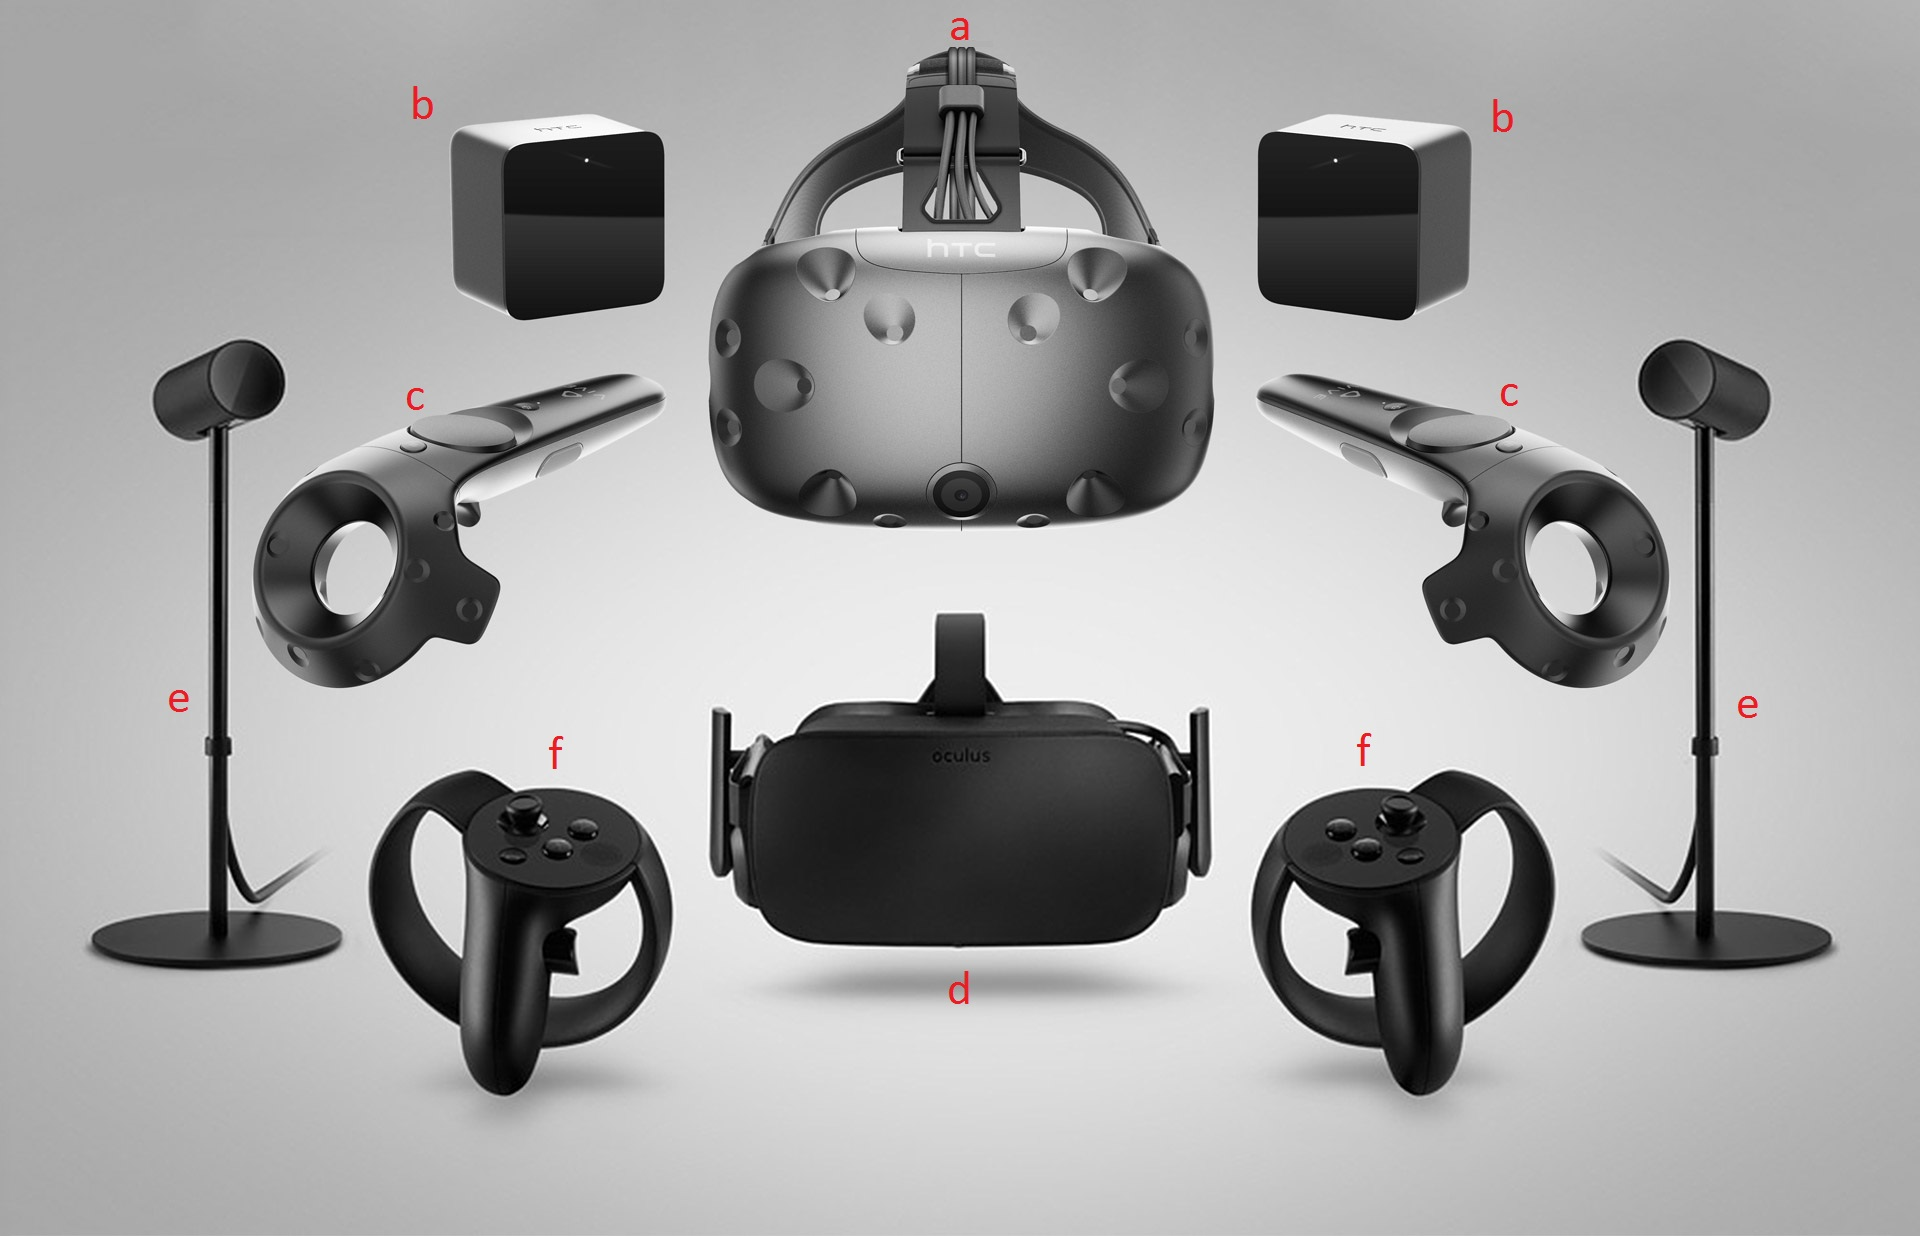
\includegraphics[width=\linewidth]{pictures/vive_and_rift_marked.jpg}
	\caption[The HTC Vive and Oculus Rift Hardware]{The HTC Vive and Oculus Rift Hardware. 
    a) The HTC Vive headset (HMD). b) The HTC Vive Lighthouse Stations. c) The HTC Vive Controllers. d) The Oculus Rift headset (HMD). e) The Oculus Rift Constellation Sensors. 
    f) The Oculus Rift Touch Controllers. Picture from \citet{ROADTOVR2016}}
	\label{fig:vive_and_rift_marked}
\end{figure} 

\section{Virtual Reality demands}
Virtual reality places some strict demands on performance and software design to avoid discomfort for the user. This is in many ways connected to how virtual reality "tricks" 
the user's brain into thinking the virtual experiences are actually real, thus giving it its "reality feel". Failing to meet these demands can quickly result in significant 
discomfort for the user, often called "virtual reality sickness", a kind of motion sickness~\citep{ARSTECHNICA2013}. Some of this demands are described below:

\subsection{Latency requirements}
Virtual reality headsets have a much stricter requirements for latency, i.e the time required for an input to have a visible effect, 
than with use of regular displays~\citep{ROADTOVR2013}. If this demand isn't met the system might feel "sluggish", and user's actions and 
visual feedback might feel disjoint, which often lead to virtual reality sickness. According to one of the engineers behind the HTC Vive, the ideal
latency is between 7 and 15 milliseconds~\citep{ARSTECHNICA2013}. One important component of this latency is the refresh rates of the displays, i.e 
how often the display hardware updates its buffers and thus "draws" a new image on the displays. As an example both the Oculus Rift CV1 and the HTC Vive
has a refresh rate of 90 Hz (i.e the display updates 90 times per second), as opposed to the 60 Hz which is more common in commodity displays.
In addition to refresh rate frame rate, i.e how often the graphics processing unit (GPU) renders frames/images, is also important. To ensure 
that the displays don't "redraws" and identical frame on a buffer update the frame rate should thus ideally be the same or higher than the refresh 
rate (e.g 90 frames per second for the Oculus Rift CV1 or HTC Vive). Refresh rate and frame rate are thus highly codependent, where performance is only as good as the weaker
of the two, and the target computer should thus have a GPU strong enough to meet a frame rate equal or above to the HMD's refresh rate. 



\section{A review of two HMD's hardware}

\subsection{The Oculus Rift CV1}

\subsection{The HTC Vive}
The HTC Vive uses more than 70 sensors \citep{BBC2015}.